\subsection{Overview}
\indent The high-level architectural diagram provided below offers a conceptual overview of the CodeKataBattle (CKB) platform's infrastructure. It delineates the system's division into three primary layers: Presentation, Application, and Data. 
\newline
\indent The Presentation Layer captures the user interaction with the system via a standard web browser, illustrating the entry point for both educators and students. \\
\indent The Application Layer is the system's backbone, housing the business logic and core functionalities, including load balancing, application servers, and interfaces for external services such as the GitHub API, Static Analysis Tool API, Email Service, and Notification Service. A dedicated firewall protects this layer, ensuring secure data transactions. It is mainly responsible for handling requests from clients and presentation layer. This layer communicates with the Data Layer, to store and process the data.\\
\indent The Data Layer is structured to manage persistent data and comprises the Database Management System (DBMS), which supports sharded databases for scalability, and a File Storage system that accommodates various data types, including educator uploads and code submissions. This layer is mainly  responsible for data storage and access by querying. \\
\indent Each component is strategically placed to optimize performance and maintainability, reinforcing the platform’s robustness and reliability. The details are discussed in the following sections.
\newline
\indent Here, it is important to explain the reasons that led to choice of 3-Tier Architecture. Firstly, this kind of separation of logic helps to improve horizontal scalability. Each layer can be developed and maintained by different software teams. Also, different technologies can be adopted for presentation, application and data layers without affecting each other. \\
\indent On the other hand, another option can be Microservice Architecture, which is more modular then the 3-layered architecture.It provides higher degree of separation between each part of your application, which leads to even more flexibility and agility than you'd get from a three-tier app. However, as a trade-off, a Microservice Architecture includes more components to deploy and track, which makes developing and maintaining application more challenging because of the higher complexity. In this scenario, even orchestrators and service meshes can be needed. When we think about the CodeKataBattle platform specifically, the scalability of 3-layered architecture is well enough with several servers. A Microservice Architecture might not make sense when a large cluster which maximizes scalability and resilience is not used. Eventhough Microservice Architecture would be better option to scale up and down in a granular way, because of such complexity , it will be excessive for the CodeKataBattle. \\

\begin{figure}[H]
    \centering
    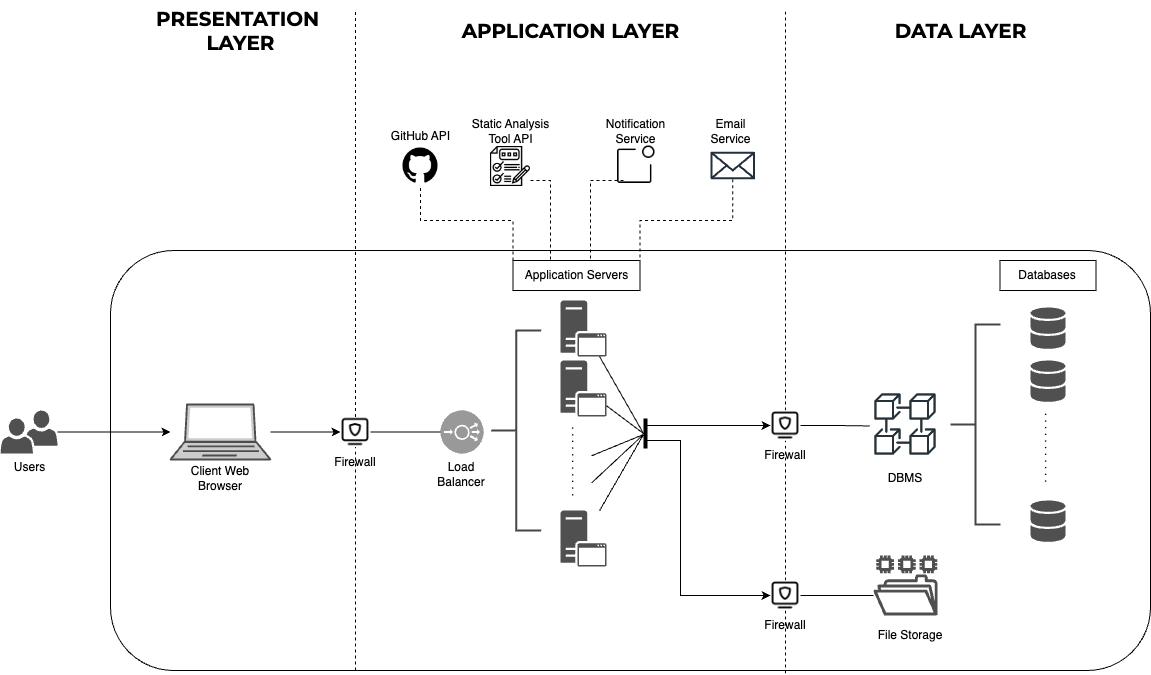
\includegraphics[scale=0.25]{Images/hl-architecture.drawio.png}
    \caption{High-Level Architecture of the System}
\end{figure}

\newpage 
\subsection{Component View}

\begin{figure}[H]
    \centering
    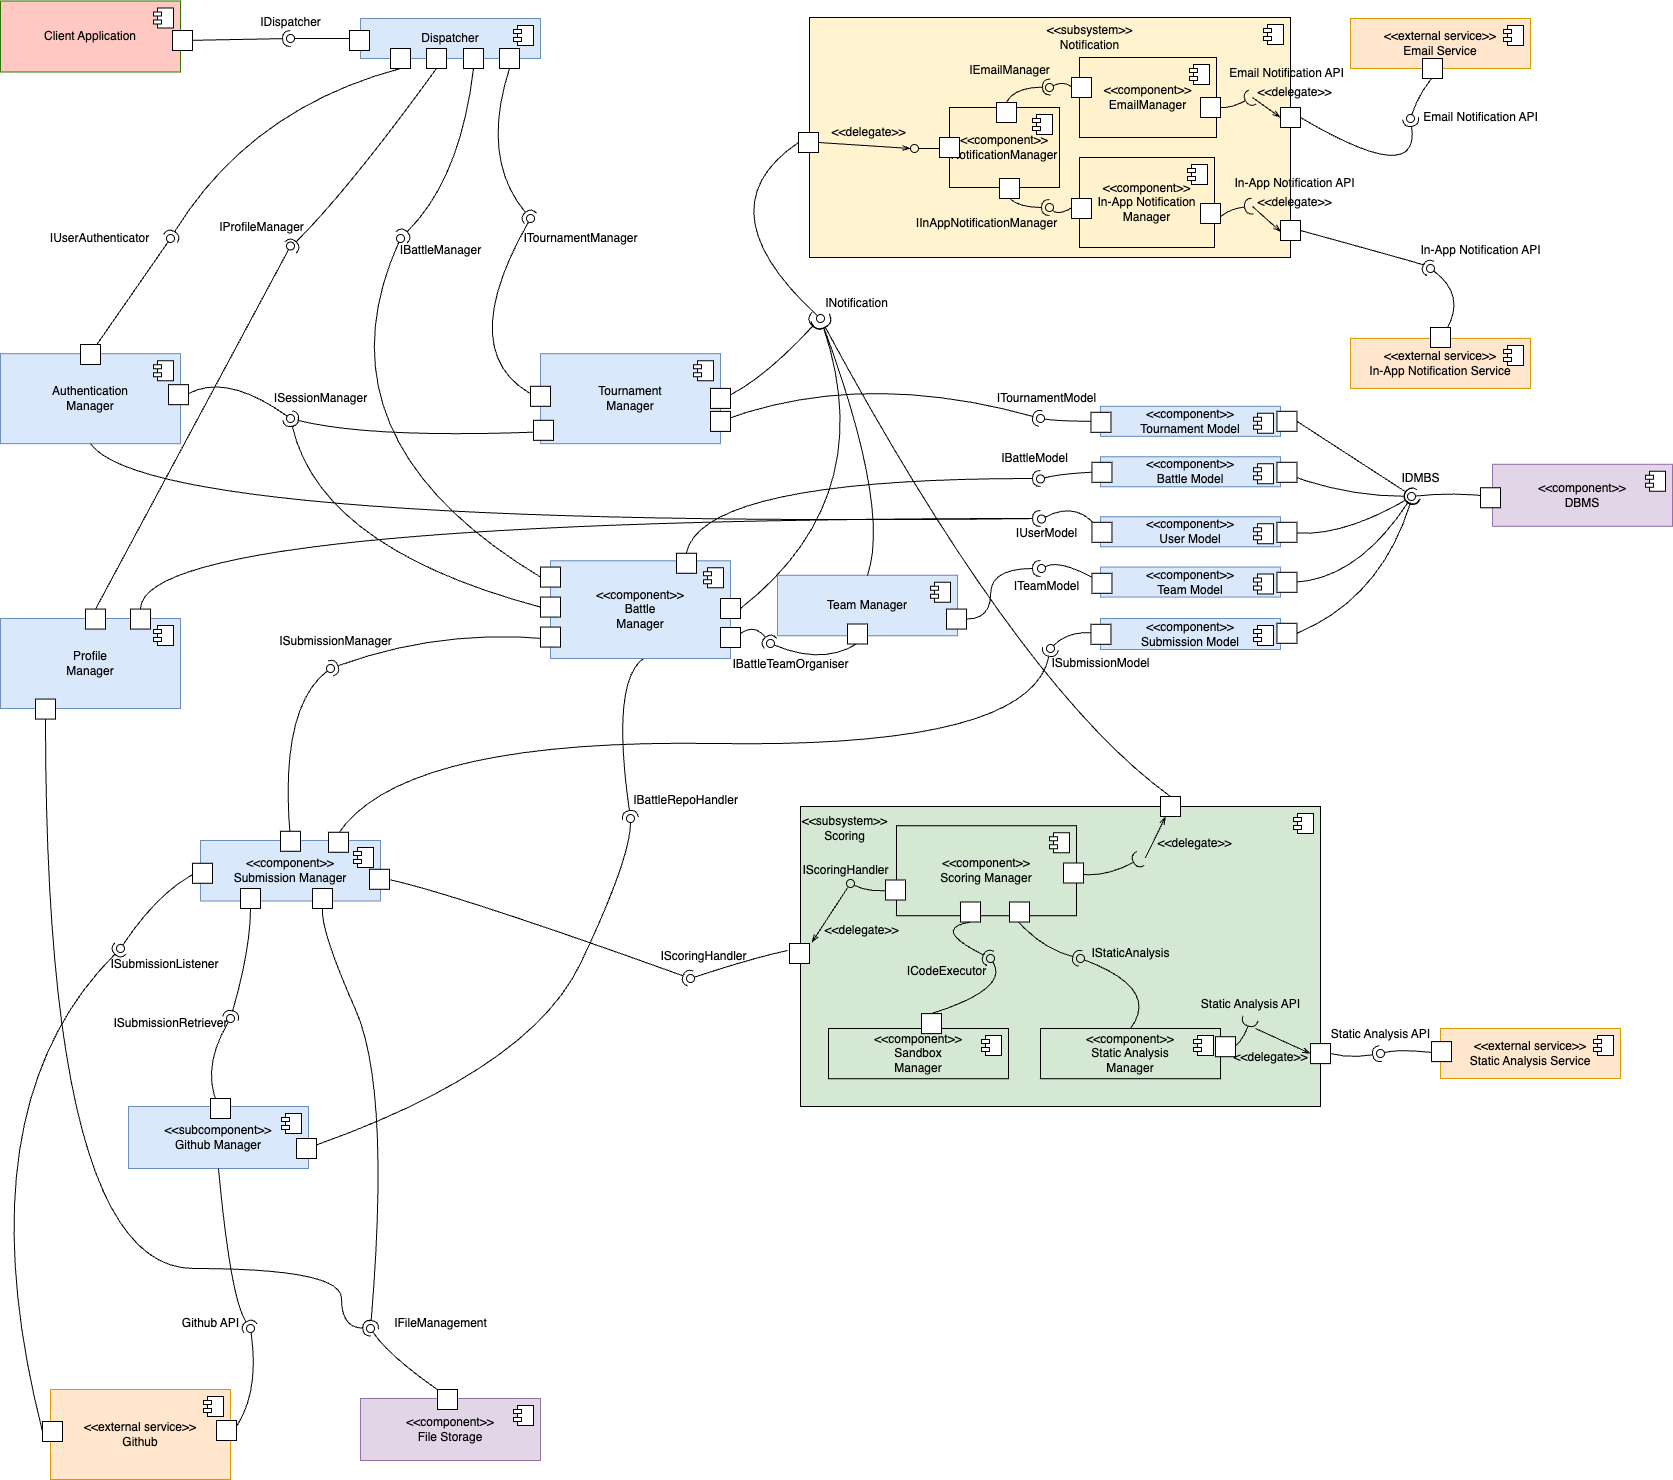
\includegraphics[width=\linewidth]{Images/DD-component.drawio.png}
    \caption{Component Diagram}
\end{figure}



\newpage
\subsection{Deployment View}
\\
\indent Our architecture mainly consists of 3 parts: 
\begin{itemize}
    \item A Static Web Server
    \item Application Server
    \item Database Server
\end{itemize},
\\
Users can interact with website via a browser and a device that has browser support such as a computer, a mobile phone etc. Content Delivery Network is used for the web server which behaves as an entry point to users. It hosts the static and dynamic web content, such as .html, .css, .js, and image files, to users. Using Content Delivery Network has some advantages in terms of performance, reliability and security. CDNs speed up content delivery by decreasing the distance between where content is stored and where it needs to go, reducing file sizes to increase load speed, optimizing server infrastructure to respond to user requests more quickly. Also  if a server, a data center, or an entire region of data centers goes down, CDNs can still deliver content from other servers in the network. Moreover, it is also very useful from the security perspective. With their many servers, CDNs are better able to absorb large amounts of traffic, even unnatural traffic spikes from a DDoS attack, than a single origin server.
\\
\indent Then we have our Application Server which is hosted on the cloud with 2-4 instances. 
\\
\indent At the Data Layer, we have database server which includes database and DBMS with a firewall. 


\begin{figure}[H]
    \centering
    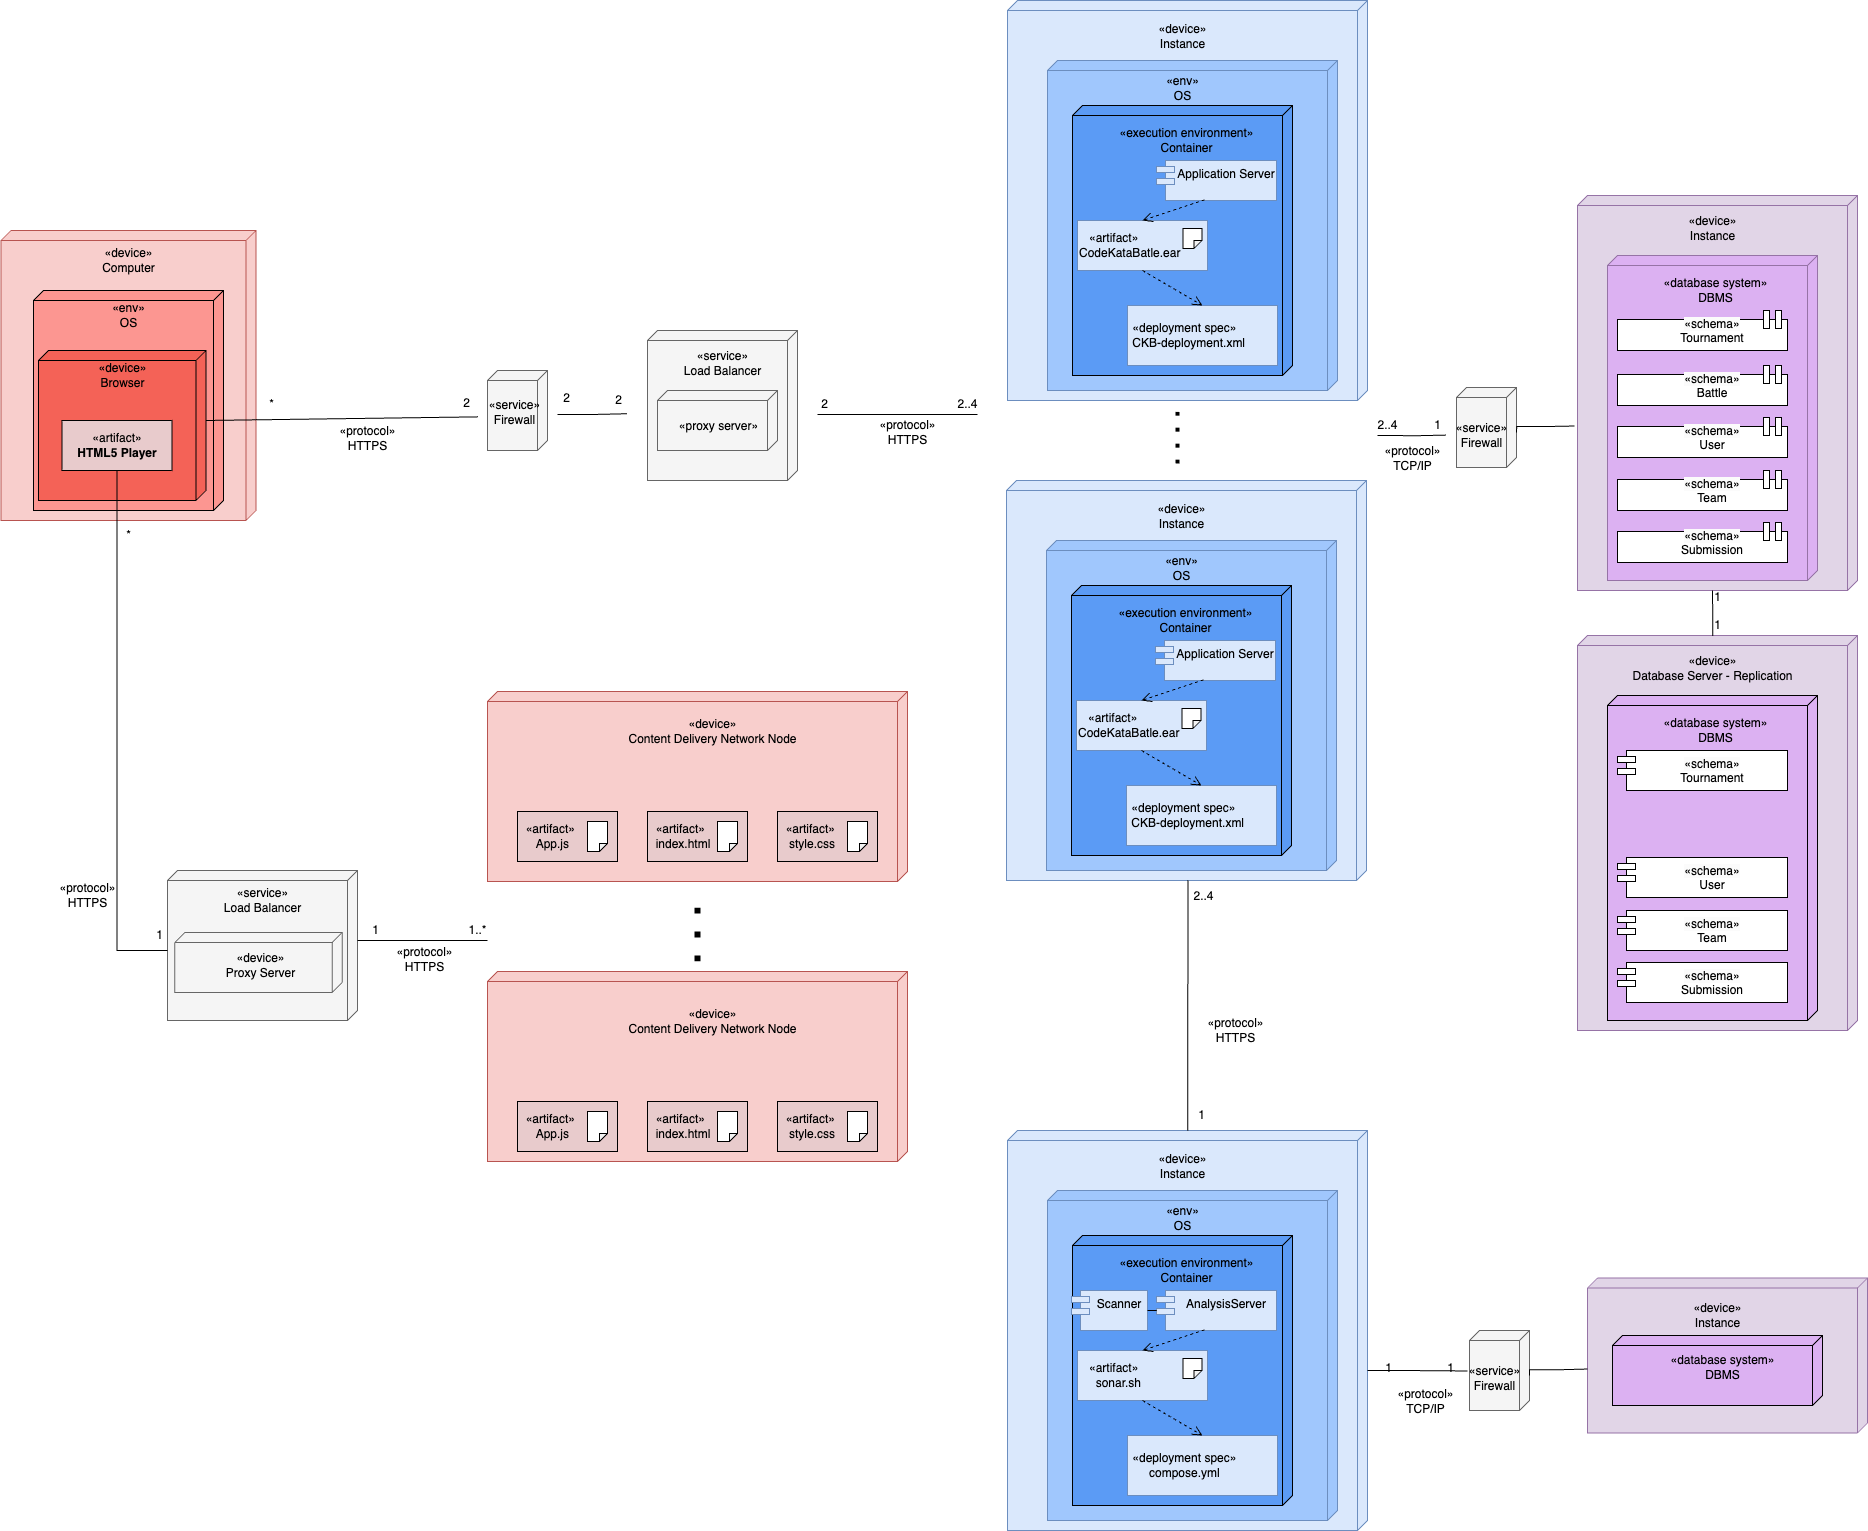
\includegraphics[scale=0.25]{Images/DD-deployment.drawio.png}
    \caption{Deployment Diagram}
\end{figure}

The deployment diagram offers a more detailed view over the hardware and software resources of the application:
\\
\indent \textbf{User Device:} User device can be any device that supports a web browser.
\\
\indent \textbf{Static Web Content:} The static web content of CodeKata Battle is hosted by Content Delivery Network with a Load Balancer distributing traffic and workload. The nodes in CDN can be scaled to very large numbers because it needs low computation power and memory. Geographically distributed nodes can be helpful to provide web interface with great performance in terms of speed. Briefly, The this content is static and all of its code is run on the
client’s machine,by browser, so there is no need for any logic to be implemented on the CDN side.
\\
\indent \textbf{Application Server:} All the business logic is handled in the Application Server which is hosted on the cloud with minimum 2 and maximum 4 instances. Obviously, these numbers can change in time but ,for an initial design, using 2-4 server instances would be adequate. Also 2 load balancer is used to distributing workload among application server instances. This is the bottleneck of the application so we decided to use 2 of them.
\\
\indent Distributing incoming requests among multiple servers hosted on the cloud can helps us to fulfill some technical constraints:
\\
\indent \textbf{Reliability}: Cloud providers often offer high reliability through redundant resources and infrastructure. If one server fails, others can take over, minimizing downtime. Regular backups and disaster recovery options further enhance reliability.

\indent \textbf{Availability}: High availability is a key feature of these kind of hosting. Multiple instances in the cloud use multiple data centers around the world, ensuring that your services remain accessible even during local outages or disruptions.

\indent \textbf{Security}: Cloud providers invest heavily in security measures, including physical security of data centers, network security, and data encryption. Monitoring tools and firewall helps to sustain a secure application server.

\indent \textbf{Scalability}: Increasing or decreasing the size and amount of the instances can help to deal with changing request loads that servers have to respond to, also with the help of load balancing. Because of the changes in traffic or workload, we would need different computation and memory capacity. You can easily scale your server resources up or down based on demand, ensuring optimal performance without overpaying for unused capacity.

\indent \textbf{Maintainability}: Cloud providers handle hardware maintenance, updates, and patches, allowing us to focus on core business and application development. Also logging and monitoring tools generally works well with this kind of hosting other than in-house hosting or custom solutions we can develop.

\indent \textbf{Portability}: Cloud environments support portability and interoperability. You can move applications and data across different cloud environments or providers with relative ease, avoiding vendor lock-in and allowing for flexibility in deployment choices.
\\
\indent \textbf{Database}: This instance contains database with necessary schemas and database managements system. It is used with a replication It is also has a replicated version of itself, because of our \textbf{reliability} and \textbf{availability} constraints. By replicating data across multiple nodes or locations, the system can ensure high \textbf{availability}. If one node fails, the others can continue to operate, minimizing downtime and ensuring continuous access to data. Also, in the event of a major failure or disaster affecting the primary data center, having replicas ensures that data is not lost and can be quickly recovered. 
\\
\indent \textbf{Firewalls:} Firewall services act as a security gatekeeper for a system's business and data layers, screening incoming connections. They enhance security by enforcing rules that either permit or block traffic, safeguarding the system from illicit access or harmful attacks.

\indent \textbf{Load Balancers:} A load balancer is employed to evenly distribute incoming traffic across various instances of an application. This strategy optimizes the use of resources, boosts performance, and maintains high availability. By doing so, the load balancer aids in managing a significant influx of requests, preventing the application from being overwhelmed or suffering downtime, and contributes to overall stability.



\subsection{Runtime View}




\subsection{Component Interfaces}



\subsection{Selected Architectural Styles and Patterns}




\subsection{Other Design Decisions}


